\documentclass[thesis.tex]{subfiles}

\chapter{Theoretical Overview \& Related Works}
\section{Machine Learning}
Machine Learning (ML) is the study of algorithms and statistical models that perform tasks without explicit instructions, but by learning and inferring from data. Machine learning algorithms produce "models" from data during their training phase, and infer the model's outputs during runtime to produce results on unseen (test) data.

Machine learning is a subfield within artificial intelligence. Most machine learning problems attempt to solve human-centric tasks, such as visual cognition, or language understanding, etc,... Since machine learning is approximate by nature, problems that would require machine learning solutions are often NP or incomputable.

\subsection{Relation to statistics}
Machine learning is closely related to statistics. A machine learning model provides prediction based on a statistical model of its training data. Although they aim to generalize to new examples, these models are still heavily bound to the training set's distribution. Understanding the statistical properties for each problem is an important step in creating accurate models.

\subsection{Relation to optimization}
Machine learning also has intimate ties to optimization: many learning problems are formulated as minimization of a loss function on the training set. The loss function represents the discrepancy between the model's predictions and the actual problem instances.

The key difference between machine learning and the above fields is their goals. Statistics and optimization both aim to extract results from the given (training) data, whereas machine learning is concerned with generalizing to unseen data.

\subsection{Basic concepts}
\subsubsection{Types of learning}
There are several types of learning algorithms, including: supervised learning, unsupervised learning, semi-supervised learning, and reinforcement learning.

Supervised algorithms learn from a dataset containing both the inputs and desired outputs (labels). The trained model contains a function that associates any given input with an output, and aims to produce correct outputs for both seen and unseen data. Two sub-types of supervised learning are regression (where the output is a continuous value) and classification (where the output is one or several discrete classes). Common supervised learning algorithms include Naive Bayes classification, Support Vector Machines (SVMs), Decision Trees and Neural Networks. This is the most common type of machine learning, used in domains such as image classification, sentiment analysis, or speech recognition, etc,...

Semi-supervised algorithms are similar, however they are designed to handle missing labels or very small datasets, often by making heuristic assumptions for the problem.

Unsupervised algorithms, on the other hand, make use of unlabeled data, where only the input is known. Often, the goal for these models is to learn a relationship between the examples. Instead of responding to feedback, unsupervised learning algorithms identify commonalities in the data and react based on the presence or absence of such commonalities in each new piece of data. Popular unsupervised methods include k-means Clustering, and Neural Autoencoders. A major application for unsupervised learning is cluster analysis, in which entities (such as users, products, etc,...) can be classified into groups based on their features.

Finally, reinforcement learning algorithms are modeled as agents within an environment. The environment provides feedback to the agent's actions, which are interpreted as reward values (Figure \ref{fig:rl-model}). The goal in reinforcement learning is to learn a policy for the agent to perform which optimizes its reward, and ultimately achieve its task. Notable applications of reinforcement learning include self-driving cars and game-playing AIs (eg. Google's AlphaGo \cite{silver2016alphago}).

\begin{figure}[htp]
	\centering
	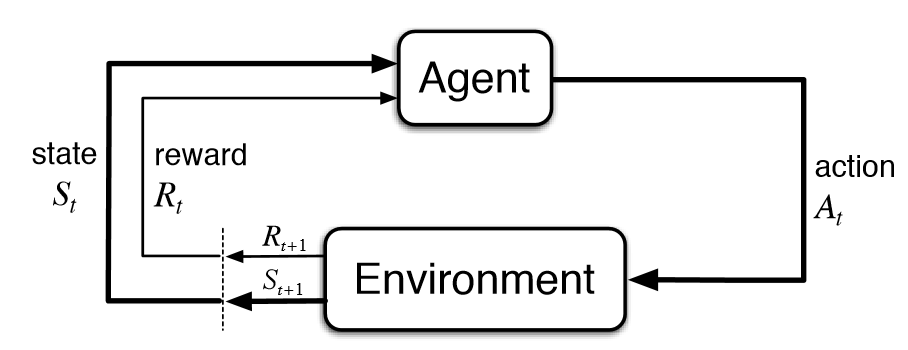
\includegraphics[width=0.75\textwidth]{rl-model.png}
	\caption{General model for reinforcement learning}
	\label{fig:rl-model}
\end{figure}

\subsubsection{Feature extraction}
A key phase in training any machine learning model is representing the training examples in a format suitable for the model. This process is called feature extraction.

Feature extraction heavily relies on both the problem domain and the algorithm being used. On one hand, an example should be represented such that there's sufficient information for models to learn, while at the same time avoiding noisy features which can cause false correlation. As an example, to train a model predicting a person's height, their weight and gender could be considered good features, while their marital status would be a bad feature. On the other hand, each ML algorithm has specific requirements and advantages in terms of input data. Naive Bayes and Decision Tree classifiers, for example, only accepts discrete values as input, while SVMs and Neural Networks only work with continous values.

Several common techniques are utilized in feature extraction:

\begin{itemize}
	\item Normalization/Scaling: To negate the effect of uneven value ranges between features, these values are often normalized to a range between 0 to 1 (or -1 to 1), with regards to the mean value for that feature.
	\item Discretization: To allow discrete models to work with continous features, discretization techniques are often applied. A common method is to split the value range into small sub-ranges.
	\item Embedding: Conversely, discrete features are often transformed into continous vectors, dubbed embedding vectors. Intuitively, embedding vectors seek to approximate the relationships between their respective discrete values (eg. relations between different words). This is often achieved using some form of unsupervised learning. The most widely used form of embedding vectors is Word2Vec \cite{mikolov2013distributed} for word representation (Figure \ref{fig:word2vec}).
\end{itemize}

\begin{figure}[htp]
	\centering
	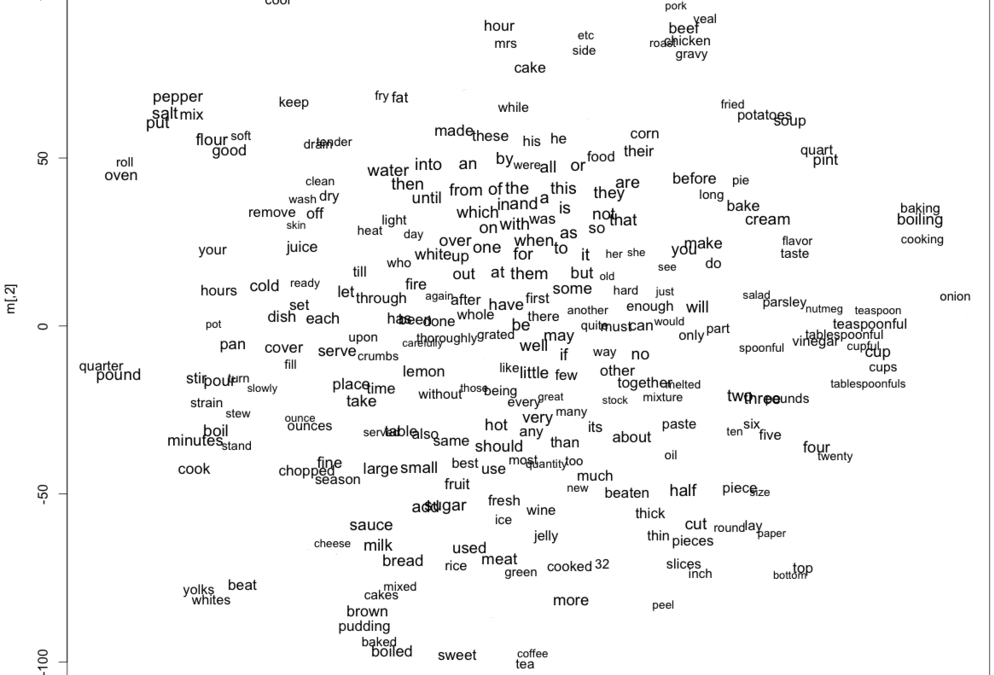
\includegraphics[width=0.9\textwidth]{word2vec.png}
	\caption{Visualization of word2vec embeddings}
	\label{fig:word2vec}
\end{figure}

\subsubsection{Partioning datasets}
Evaluating the effectiveness of ML models differ from other algorithms and statistical models. In this section, we focus on evaluating supervised models.

Supervised ML models are trained on a training dataset, however the goal is to produce accurate predictions on unseen data outside this training set. Hence, it's impossible to evaluate on training data, otherwise a model that "learns" by simply memorizing the training set would score perfectly, yet unusable. As such, a subset of labeled data is set aside from training as the test dataset, which only serves to evaluate the model.

Additionally, many models have hyperparameters that require selection, often by experiment. This selection should also be done on unseen data, yet it's unfair to use the test set as this simply picks out whichever parameter set that happens to fit the test distribution. Instead, a seperate validation dataset is held out for this purpose.

For large datasets, a straightforward split of 3 datasets is often made with a ratio of around 70/15/15 for training, validation and testing. In smaller datasets, an alternate approach is $k$-fold cross validation, where the entire dataset is split into $k$ equal parts (folds). Training is then performed $k$ times, each using one fold as the validation and test set, and the rest as the training set. Evaluation results are then averaged among all runs.

When splitting datasets, it can sometimes be important to maintain the distribution of classes or other feature properties in the original data. This technique is called stratified sampling, and is especially critical for datasets that are unevenly distributed.

\subsubsection{Evaluation metrics}
Different metrics are used to evaluate machine learning models, depending on the problem domain. Most often, metrics focus on how accurate the model is in performing the given task, however can also include other requirements like efficiency, robustness, scalability or interpretability.

For classification models, the most common metric is accuracy, which measures the ratio of correct classifications made by the model. However, this metric can be noisy on unbalanced datasets. Specifically, if $90\%$ of the dataset belongs to class A, then a classifier that always predicts class A would have $90\%$ accuracy (!). Therefore, 3 other metrics are usually added to evaluation: precision, recall, and F1 score.

Precision measures the ratio between true positives (number of accurate predictions made by the model for one class) to all predictions in that class. Recall measures the ratio between true positives for a class and all examples labeled as that class. Finally, F1 score is the harmonic mean between precision and recall. Calculating these metrics is often done using a confusion matrix (Figure \ref{fig:confusion-mat}).

\begin{figure}[htp]
	\centering
	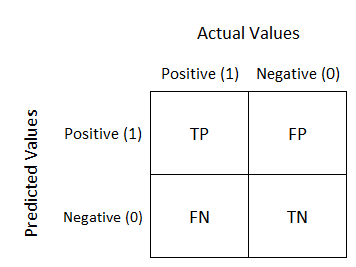
\includegraphics[width=0.5\textwidth]{confusion-mat.png}
	\caption{A confusion matrix}
	\label{fig:confusion-mat}
\end{figure}

In essence, precision measures how likely each 

\section{Neural Networks \& Deep Learning}
\subsection{Object Detection With Convolutional Neural Networks}

\section{Computational Graphs \& Deep Learning Frameworks}
\subsection{Computational Graphs}
Although they are commonly visualized as layers of neurons, neural networks are more often represented as computational graphs.

Computational graphs are directed graphs that express a series of computations. Each node is either an input variable, or, when there are incoming edges, a function of those edges' tail nodes. Edges simply denote dependencies between nodes (eg. $a = b + c$).

\begin{figure}[htp]
	\centering
	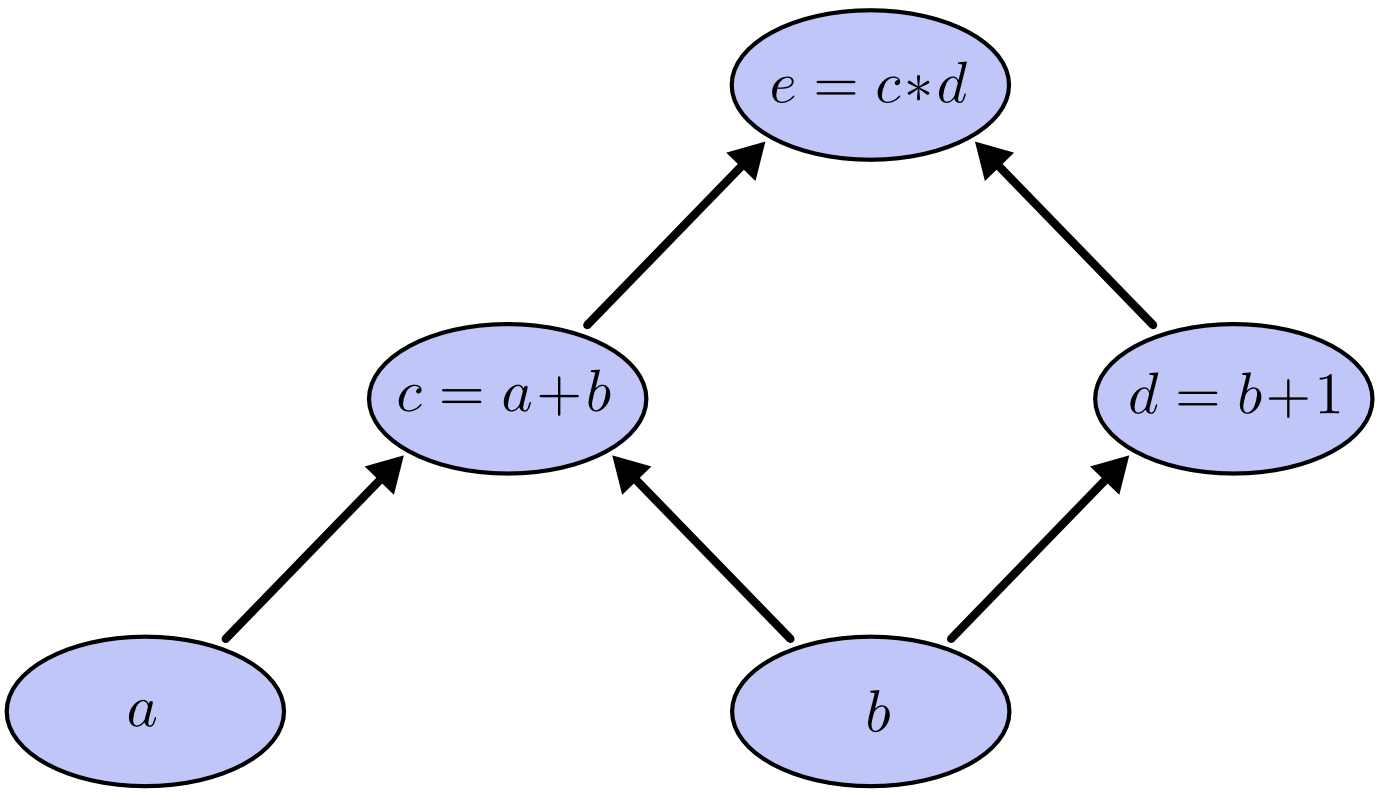
\includegraphics[width=0.5\textwidth]{cgraph1.png}
	\caption{An example computational graph with inputs $a$, $b$ and outputs $(a + b)(b + 1)$}
	\label{fig:cgraph1}
\end{figure}

It is trivial to traverse the graph from all input nodes to calculate its outputs. If we model a neural network as a series of computations (eg. $y = sigmoid(x \cdot w)$), then this corresponds to the network's forward pass. Conversely, since each node knows about its outcoming edges and operator, it can infer the gradient w.r.t each edge. In other words, we can calculate gradients at each node automatically, by traversing the graph backwards. This is immensely helpful for backpropagation, which requires the gradient for each neuron to be calculated.

\begin{figure}[htp]
	\centering
	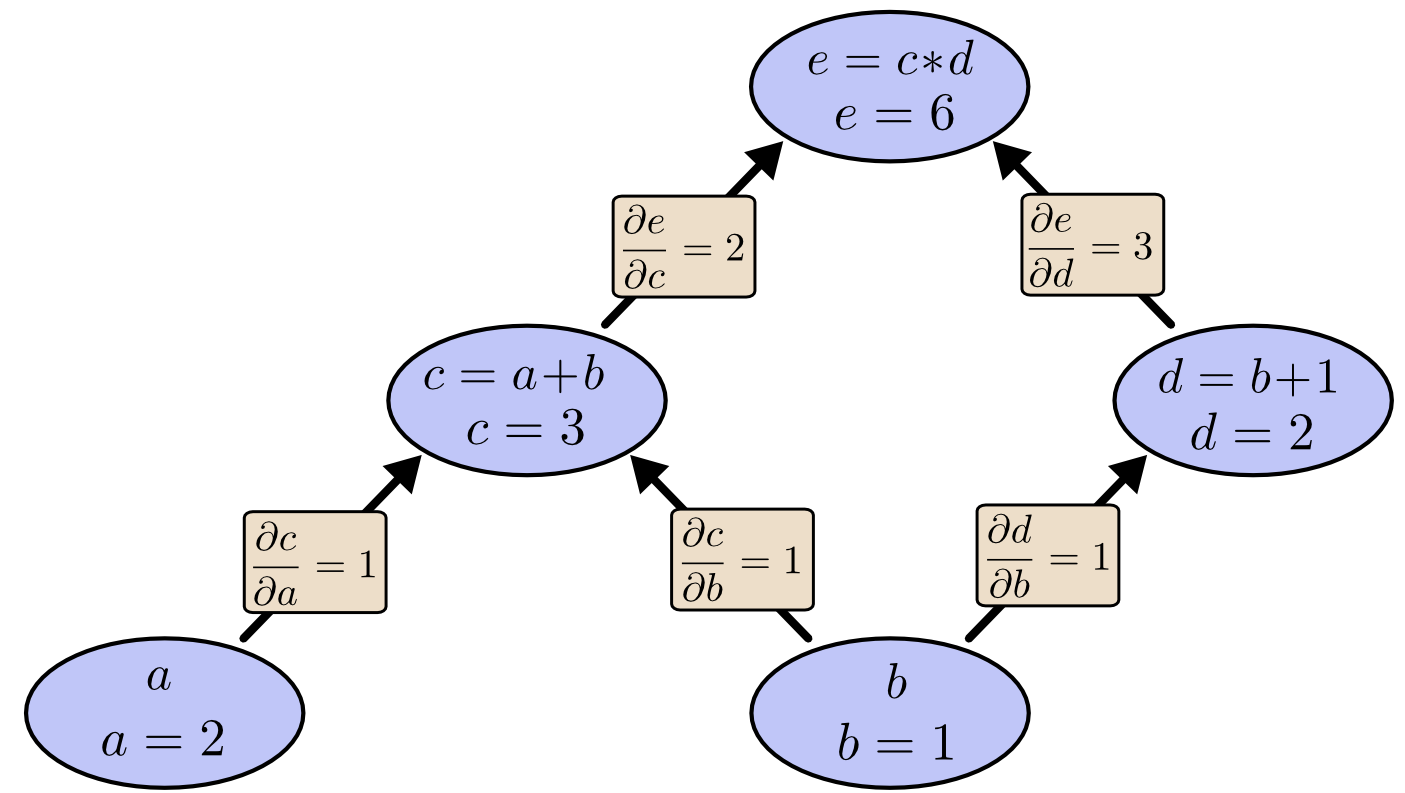
\includegraphics[width=0.5\textwidth]{cgraph2.png}
	\caption{Calculating gradients on each edge}
	\label{fig:cgraph2}
\end{figure}

The fact that neural networks can be modeled as computational graphs has several implications. Most significantly, it means that backpropagation can be done automatically, assuming each op is differentiable. This greatly reduces the amount of work required when designing network architectures, as only the forward pass need to be defined. Moreover, graph optimization methods can be applied to their architectures, allowing them to be more compact and efficient.

\subsection{Deep Learning Frameworks} \label{section:dlframeworks}
The use of computational graphs for deep learning became prevalent in part due to the multiple frameworks that leverage them for automatic gradient calculations. Two of the earliest were Theano (2010) \cite{bergstra2010theano} and Caffe (2014) \cite{jia2014caffe}, followed by Google's TensorFlow (2016) \cite{abadi2016tensorflow}, which remains the most popular framework to date. These tools define the same 2-phase workflow for running neural networks: the first phase where the computational graph is symbolically defined, and the second phase where numerical input is fed to the runtime to execute the graph.

By seperating graph definition and the actual runtime, these early frameworks can apply several optimizations during graph "compilation". This also helps improve performance, since definition is often done in the Python language, while the runtime can be written in lower-level, more performant languages (eg. C, C++,...). Finally, since the graph is finalized after compilation and is essentially data, they are portable and serializable, which helps deployment at scale.

On the other hand, compiled graphs are often criticized for their steep learning curve and being difficult to debug. Since the framework runtime completely takes over execution and even modifies the graph during optimization, it's often difficult to keep track of results and errors. This motivated the creation of dynamic graph frameworks, most notably PyTorch (2017) \cite{paszke2017pytorch} and Chainer (2015) \cite{tokui2015chainer}. These frameworks simply constructs graphs \emph{on the go}, alongside the actual calculations. This has the benefit of being easier to grasp, and operations can be transparently observed instead of obscured during execution. However, they suffer from fewer optimizations and lower portablility.

Despite their differences, static and dynamic graph frameworks have shown a tendency to overlap in recent years. Namely, TensorFlow 2.0 introduced Eager Execution, which attempts to create a smoother, dynamic experimental workflow. In contrast, PyTorch 1.0 added Script Mode in order to support compiled graphs, a feature that used to be delegated to conversion to Caffe 2. In the end, we can expect these libraries to provide both an intuitive development experience and optimized for production.

On top of these frameworks, multiple tools and interfaces have been proposed in recent years to help simplifying their workflow. High-level libraries like Keras \cite{chollet2015keras} allows intermediate users to interact more easily with TensorFlow, Theano and CNTK, while tools such as NVIDIA DIGITS create a streamlined workflow for multiple frameworks.

\section{Training Neural Networks in Parallel}
A major drawback for deep neural networks is the computational complexity of training them. LeNet (1998) \cite{lecun1998lenet}, for example, has over 100,000 parameters, while ResNet-50 (2016) \cite{he2016resnet} has 25 million. Optimizing these parameters over many iterations is very computationally intensive, and training even a small network such as LeNet could take several days on standard CPUs.

From a parallel computing perspective, optimizing neural networks has a lot of potential optimizations. A common approach is running training examples in parallel. In each iteration, gradients are calculated for different data batches in each node, then reduced into the final update values for the model. The reduce procedure is critical in this approach, as it determines the communication overhead for each iteration. The most straightforward method would be using master nodes (often denoted parameter servers), where gradients are collected and reduced. However, this creates a bottleneck at the parameter servers themselves, and forces another level of communication if multiple parameter servers are used. 

\begin{figure}[htp]
	\centering
	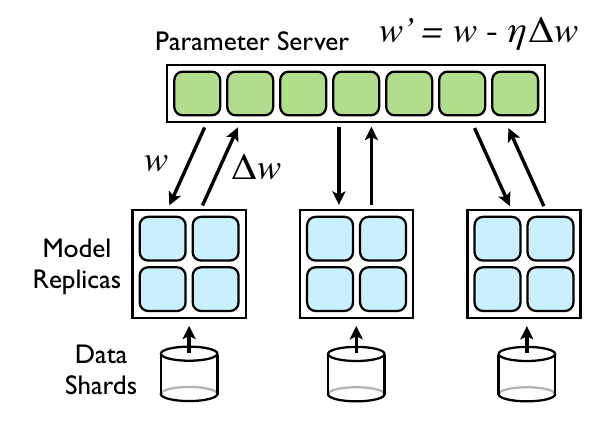
\includegraphics[width=0.7\textwidth]{allreduce.png}
	\caption{Centralized Allreduce with Parameter Server}
	\label{fig:allreduce}
\end{figure}

A more efficient method called "Ring Allreduce" was proposed by researchers at Baidu \cite{baiduAllreduce}. As the name suggests, this method places nodes sequentially into a "ring". When the reduce operation is called, the first node sends its gradient to node 2, where it's reduced with node 2's gradient. This result is then sent to node 3 and so on. When all nodes are reached, node 1 would contain the final gradient. We would then make another pass around the ring to update all nodes with the new gradient.

Something to take note of is the effect of this paradigm on the training results itself. Since we are running each replica on different batches, the model is essentially training with a larger batch size. Multiple works, for example \cite{chen2012pipelined}, have observed that huge batches can hinder a network's learning process, especially in early iterations. This puts somewhat of an upper limit to the scalability of this approach.

\begin{figure}[htp]
	\centering
	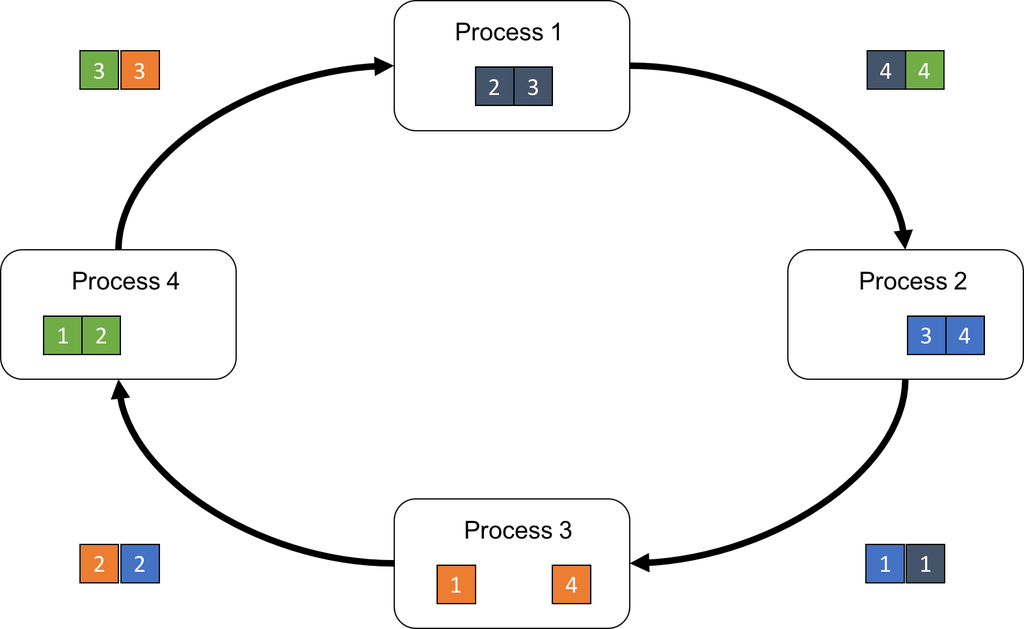
\includegraphics[width=0.7\textwidth]{ring_allreduce.png}
	\caption{Ring Allreduce}
	\label{fig:ring_allreduce}
\end{figure}
\FloatBarrier

Another approach, as implemented by the authors of the DistBelief framework \cite{dean2012large}, is to distribute the network graph vertically on multiple nodes (Figure \ref{fig:model_parallel}). This "striping" appproach avoids constant synchronization between nodes, but also only applicable to large, wide networks whose layers can be efficiently split.

\begin{figure}[htp]
	\centering
	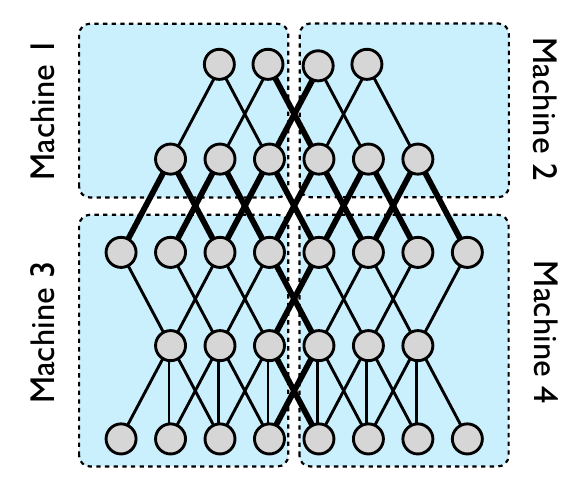
\includegraphics[width=0.7\textwidth]{model_parallel.png}
	\caption{Model parallelism in DistBelief \cite{dean2012large}}
	\label{fig:model_parallel}
\end{figure}

Finally, a strategy called "pipeline backpropagation" was investigated by the authors in \cite{petrowski1993performance}. The idea is similar to striping, where the network graph is distributed across nodes. However, this method partitions the graph horizontally, where each node contains one or several full layers, forming a data pipeline. During training, each node works independently on their own data, disregarding the current state of the whole graph. Updates are performed with a delay, which become more noticeable at deeper layers of the network.

\subsection{Using Graphics Processing Units}
A breakthrough for training DNNs was the use of Graphic Processing Units (GPUs), as first presented by Raina et al \cite{raina2009gpu} in 2009. Similar to graphics processing, neural networks are trained using operations on large matrices, which benefit from GPUs' multi-core design. Since then, the toolchain for GPU-accelerated neural network has matured significantly. Libraries such as CUDA, CUDNN \cite{chetlur2014cudnn}, and high level interfaces have made training of neural networks on GPUs trivial.

All of the frameworks mentioned in \ref{section:dlframeworks} allows execution on GPUs, the majority of which rely on NVIDIA's CUDA and CUDNN libraries.

\subsection{Using Computing Clusters}
While GPUs have greatly improved DNN training speed, modern networks continue to be even more complex, along with larger training datasets. This requires more scalable training mechanisms, particularly on multiple devices. One approach, as seen with Google's Tensor Processing Units (TPUs) \cite{jouppi2017datacenter}, is building custom hardware that are designed to work as clusters. Indeed, TPUs are very efficient and performant. However, this approach is expensive and requires a lot of effort for deployment. A more compact, user-friendly approach is to make use of existing GPUs and computer architectures. This can be done using a software layer that handles communication between GPUs/CPUs on different machines.

Support for multi-node and multi-GPU training are available in most DL frameworks, most notably TensorFlow (which utilizes Google's gRPC protocol) and PyTorch (which support several communication backends, including the popular MPI \cite{Forum:1994:MMI:898758} interface). Both implement parallelization using the data parallel approach (with Allreduce), as this is the most general solution that can apply to most neural networks.

In 2018, researchers at Uber released Horovod \cite{DBLP:journals/corr/abs-1802-05799}, a library providing a unified interface for parallel training with TensorFlow, Keras, PyTorch and MXNet. Horovod utilizes MPI for communication, and implements Baidu's Ring Allreduce. Horovod's notable feature is that it requires minimal changes to existing single-node codebases.
